\doubleSpacing
\chapter{Background}

\section{Abstract Syntax Tree}
 An Abstract Syntax Tree (AST) is a tree representation of the  source code written in a programming language. It is usually the result of the syntax analysis phase and serves as an intermediate representation of the program. 
AST starts with a root node and it contains child nodes. A terminal node in AST is either an identifier or a constant. The typical implementation of an AST makes large use of polymorphism. The nodes within the AST are usually implemented with a variety of classes, all deriving from a typical ASTNode class. For every syntactic construct within the language, there'll be a class for representing that construct within the AST, like ConstantNode, VariableNode, AssignmentNode, ExpressionNode, etc. A ConstantNode doesn't contain any children, an AssignmentNode must have two and an ExpressionBlockNode will have several children.
%Self reading over. There is no critical bug
%PG- 0
%Author @rahul
\begin{itemize}
	\item \textbf{Root Node}
The node at the top of the tree is called root. If node n1 is root, it doesn't have any parent. There is only one root per tree and one path from root node to any node. The path is the connection between two nodes. In AST root node may be Classes, Enumdatatype, Interface, etc.
\item \textbf{Internal Node}
If there is a parent and child for a node then it is called internal nodes. Node n1 is the parent of node n2, if n1 is an ancestor of node n2 and is
connected to node n2. Node n2 is called a child of node n1. Nodes having the same parent are called siblings. In AST, operators/keywords are internal nodes.
\item \textbf{Leaf Node}
Nodes with no children are called leaf nodes. In AST operands are located in leaf node. In order to implement a single assignment statement(eg:x=10) there are three types of AST nodes, namely operator node(=), identifier node(x), literal node(10). The AST representation of an if-statement is shown in Figure \ref{Fig:1}
\end{itemize}

 

 
 \begin{figure}[H]
 	
 	
 	\centering
 	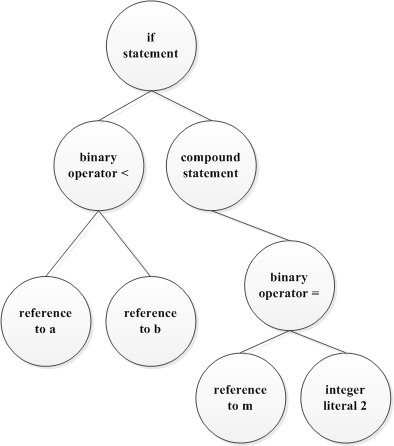
\includegraphics[width=.6\linewidth]{Figures/image1}
 	\caption{AST of  if(a\textless b) m=2}
 	\label{Fig:1}\cite{}
 	
 \end{figure}

 \subsection{AST Traversing}
 
\subsubsection{Visitor pattern} 
 A compiler that parses a program and represents it as an AST. It has various
 kinds of nodes like Assignment, Variable Reference, Arithmetic
 Expression nodes, etc. Operations that one would really like to perform on the AST are type checking, code generation, variable declaration, syntax analysis, etc. These actions  should handle each type of node separately. One solution  is to define each operation in a separate node class(Figure \ref{Fig:2}). The problems with this approach are firstly it can be a confusing and time-consuming process. Secondly adding new operations require changes to all of the node classes. To solve this problem an alternative method visitor pattern is used\cite{ood}.  
 
  \begin{figure}[H]
  	
  	
  	\centering
  	\includegraphics[width=.6\linewidth]{Figures/nav}
  	\caption{Operations in separate node class}
  	\label{Fig:2} 
  	
  \end{figure}
 
 
 The Visitor pattern\cite{ood} was introduced to address the above problem. It lets us to define a new operation without changing the classes of the elements on which it operates.
  Instead of spreading all the code for a given traversal throughout the nodes classes, the code is concentrated in a particular traversal class(visitor class).  That is, encapsulate a desired operation in a separate object, called a visitor. Then the visitor object will traverse the nodes of the tree. The structure of Visitor Pattern is shown in Figure \ref{Fig:4}
  \begin{figure}[H]
  	
  	
  	\centering
  	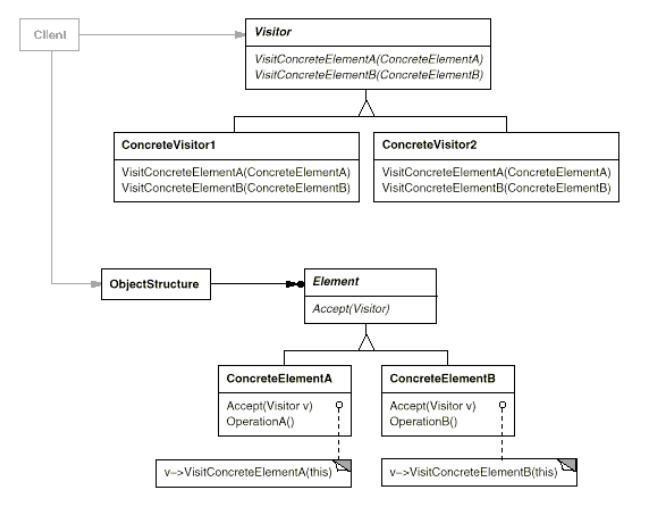
\includegraphics[width=.6\linewidth]{Figures/vstr}
  	\caption{Structure of Visitor Pattern}
  	\label{Fig:4}\cite{ood} 
  	
  \end{figure}
  The participants classes in this pattern are:
  \begin{itemize}
  	\item \textbf{Visitor} It is used to declare the visit operations for all the types of visitable classes. Normally, the name of the operation remains the same and these operations are differentiated by the method signature. The input object type decides which of the method to be called.  Visitor is implemented with the help of interface or an abstract class
  
  \item \textbf{ConcreteVisitor} For each type of visitor, all the visit methods declared in abstract visitor must be implemented. Each Visitor is responsible for different operations. ConcreteVisitor implements each operation declared by Visitor.  Each operation executes a piece of the
  algorithm defined for the corresponding class
  of the object in the structure. ConcreteVisitor provides the context for the algorithm and stores its local state.
  
  \item \textbf{Visitable} This is the entry point which enables an object to be "visited" by the visitor object. Each object from a collection should implement this abstraction in order to be able to visit.
  
  \item \textbf{ConcreteVisitable} Those classes implements the Visitable interface or class and defines the accept operation. The visitor object is passed to this object using the accept operation. 
  
  \item \textbf{ObjectStructure} This is a class containing all the objects that can be visited. It offers a mechanism to iterate through all the elements. This structure is not necessarily a collection. It can be a complex structure, such as a composite object.
\end{itemize}
 The participants classes are shown in Figure \ref{Fig:3}
 \begin{figure}[H]
 	
 	
 	\centering
 	\includegraphics[width=.6\linewidth]{Figures/vis}
 	\caption{Visitor Pattern}
 	\label{Fig:3} 
 	
 \end{figure}

 
 \subsubsection{Advantages}
  Some benefits of Visitor Pattern are
  \begin{itemize}
  	\item It allows to add operations to a structure without changing the structure itself
   \item Adding new operations is relatively easy
   \item The code for operations performed by the Visitor is centralized so editing and adding new code is easy.
   
\end{itemize}
\subsubsection{Applications of Visitor Pattern}
 
  \begin{itemize}
  	\item It is applicable when similar operations have to be performed on objects of different types grouped in a structure  
 
 
 \item There are many distinct and unrelated operations needed to be performed. Visitor pattern allows creating a separate visitor concrete class for each type of operation. It separates this operation implementation from the object structure.
 
 
 \item The object structure is not likely to be changed but is very probable to have new operations which have to be added. Since the pattern separates the visitor (representing operations, algorithms, behaviors) from the object structure it's very easy to add new visitors as long as the structure remains unchanged.
\end{itemize}
 \section{Secure Coding Guidelines}

 MITRE has listed almost 700 different kinds of software weaknesses in their CWE project\cite. These
 are all different ways that software developers can make mistakes that lead to vulnerability. Most of the developers are not aware of these weaknesses. In olden days, software industry didn't care much about secure coding standards because lack of time, lack of security standards and no extra payment
 from the client, but currently, programmers started developing software systems by following secure coding standards.
 Secure code review is the process of auditing the source code for an application to verify that
 the proper security controls are present and they are invoked in the right places. Security code
 review is a way of ensuring that the application has a self-defending capability.
 
 Building secure software requires a basic understanding of security guidelines. The goal of software
 security is to maintain the confidentiality, integrity, and availability of information resources in order
 to enable successful operations. This goal is accomplished through the implementation of security
 controls. An essential element of secure software development is well-documented and enforceable
 coding standards. Coding standards encourage programmers to follow a uniform set of rules and
 guidelines determined by the requirements of the project and organization, rather than by the
 programmers familiarity or preference. Once established, these standards can be used as a metric
 to evaluate source code.
 There are many secure coding standards present in the software industry. Some of them are,
 
 \subsection{MISRA}
 MISRA\cite{misra} coding standards have been adopted by industries for developing safety-related electronic systems in road vehicles, telecom, aerospace and other embedded systems. They have separate guidelines for C and C++.  MISRA is not an open standard, so the implementers have to pay for the guideline documents. MISRA-C:2012 contains 143 rules and 16 directives. Each of the rules are classified as "mandatory", "required", or "advisory" based on the severity. Another way the rules are classified as Decidable or Undecidable. Coverity Static Analysis, Eclair, GrammaTech, Goanna are some tools for verifying MISRA standard.
 
 
  \subsection{CERT Secure Coding}
 The CERT\cite{cert-c} Secure Coding Standard provides rules and recommendations (collectively called guide-
 lines) for secure coding in the programming language. It has separate guidelines for C, C++, Java, Android Java. The goal of these rules and recommendations is to develop safe, reliable, and secure systems. For C 194 Rules and 77 Recommendations and for Java 122 Rules and 180 Recommendations. Coverity Static Analysis, Eclair, Rosechecker are some tools for verifying CERT standard.
 
 \subsection{OWASP}
 The OWASP is an online community which creates a coding standard, documentation, tools, for web application security which deals specifically with the security of websites, web applications, and web services. OWASP supports various security-related projects, one of the most popular is the OWASP Top 10. It is a famous web application security by identifying some of the most critical risks, provides examples, and offers suggestions on how to avoid it. The Top 10 vulnerabilities are Injection, Broken Authentication and Session Management, Cross Site Scripting, Insecure Direct Object References, Security Misconfiguration, Sensitive Data Exposure, Missing Function Level Access Control, Cross Site Request Forgery (CSRF), Using Components with Known Vulnerabilities, Unvalidated Redirects and Forwards. These Top 10 is referenced by many standards, books, tools, and organizations.
\section{Static Analysis of Source Code}\cite{chess2007secure}
The analysis of code without executing is called static analysis. Automated tools simplify the overhead of a static code analysis. By examining the code itself, static analysis tools can often point to the
root cause of a security problem. This is
particularly important for making sure that vulnerabilities are fixed
before the program is run for the first time. In secure coding static analysis tools are now common one which will catch the coding standard violations before execution. While typing itself some tools integrated with the text editor figure out the error.  It will help to prevent the common coding vulnerabilities like buffer overflow, cross-site scripting, SQL injection etc.

There are some problems with static analysis tools, the main ones are false positive and false negatives. False positive is a problem reported in a program when no problem actually
exists. A large number of false positives can cause real difficulties. It will increase the workload of the programmer, unwanted wastage of time and effort for correction. With a false negative, a problem exists in the
program, but the tool does not report it. The penalty for a false
negative is more danger. What is the severity of a particular violation, it will happen in future. So the false negatives are much worse. All static analysis tools are guaranteed to produce some false positives
or some false negatives or both.
\subsection{Solving Problems with Static Analysis}

Static analysis tool will address the following problems
\subsubsection{Type checking}
The most widely used form of static analysis. Many programmers don’t give
type checking much thought. Type checking
eliminates entire categories of programming mistakes. For example, it prevents programmers from accidentally assigning integral values to object
variables. By catching errors at compile time, type checking prevents runtime errors.
\subsubsection{Style checking}
Style checkers are also static analysis tools. Pure style checkers
enforce rules related to whitespace, naming, deprecated functions, commenting, program structure, and the like. Because many programmers are
fiercely attached to their own version of the good style, most style checkers are
quite flexible about the set of rules they enforce. The errors produced by
style checkers often affect the readability and the maintainability of the
code but do not indicate that a particular error will occur when the program runs.
\subsubsection{Program understanding}
Program understanding tools help users make sense of a large codebase.
Integrated development environments (IDEs) always include at least some program understanding functionality. More advanced analysis can support automatic program-refactoring features, such as renaming variables or splitting a single function into multiple
functions. Higher-level program understanding tools try to help programmers gain insight into the way a program works.  
\subsubsection{Bug finding}
The purpose of a bug finding tool is to find the violation of rules, a bug finder simply points out places where the program will behave in a way that the programmer did not intend. Most bug finders are easy to use because they come pre-defined with a set of rules that describe patterns in code that often indicate bugs.
\subsubsection{Security review}
Security focused static analysis tools use many of the same techniques found in other tools, but they are more focused on identifying security problems. There are many secure coding standards (CERT, OWASP etc)and they defined a set of rules. Security review will verify whether the programmer followed the coding standard.
 